\documentclass[11pt]{article}
\usepackage{fullpage,amsthm,amsfonts,amssymb,epsfig,amsmath,times,amsthm}
\usepackage{algpseudocode}
\usepackage{hyperref}
\usepackage{pgfplots}

\newtheorem{theorem}{Theorem}
\newtheorem{claim}[theorem]{Claim}
\newtheorem*{solution}{Solution}

\begin{document}
% PUT YOUR INFORMATION IN THESE TWO LINES 
\hfill Isai  Lopez Rodas  

\hfill 1605542, ilopezro@ucsc.edu

\begin{center}
{\bf\Large 
CMPS 102 --- Spring 2020 --  Homework 1 }
\end{center}

\begin{center}
Updated Ver. 5(04-08)\\
Three problems, 17 points, due Friday April 10 (11:59 PM) on Gradescope. 
\end{center}

%\newcommand{\set}[1]{\{ #1 \}}
%\newcommand{\qed}{ \large \hfill $\Box$ \\ \medskip }
%\newcommand{\qedq}{ \large \hfill $\Box$?? \\ \medskip }

\renewcommand{\P}{\mbox{IH}}
Before you begin the assignment, please read the following carefully.
\begin{itemize}
    \item Read the \emph{Homework Guidelines}.
    \item Every part of each question begins on a new page. Do not change this.
    \item This does not mean that you should write a full page for every question. Your answers should be short and precise. Lengthy and wordy answers will lose points.
    \item Do not change the format of this document. Simply type your answers as directed.
    \item You are \textbf{not} allowed to work in teams.
\end{itemize}
%Complete the following.
\emph{I have read and agree to the collaboration policy.}  -- Isai Lopez, ilopezro@ucsc.edu
% replacing "FirstName LastName, email@ucsc.edu" with your information.
\\
Collaborators: None%write the name of the collaborators. If you worked by yourself, please write 'none'.
\\
\hrule
\begin{enumerate}
\item (Total: 8 pts) A grad student comes up with the following algorithm to sort an array $A[1..n]$ that works by first sorting the first 2/3rds of the array, then sorting the last 2/3rds of the (resulting) array,
and finally sorting the first 2/3rds of the new array.

\begin{algorithmic}[1]
\Function{G-sort}{$A$, $n$} \Comment {takes as input an array of $n$ numbers, $A[1..n]$}
	\State G-sort-recurse($A$, 1, $n$)
\EndFunction

 \Function {G-sort-recurse}{$A$, $\ell$, $u$} % \Comment {sort subarray $A[\ell..\u]$ } 
\If {$u - \ell \leq 0$} 
	\State return \Comment{1 or fewer elements already sorted}
\ElsIf{$u-\ell = 1$} \Comment{2 elements}
	\If {$A[u] < A[\ell]$ } \Comment{swap values}
		\State  temp $\gets A[u]$
		\State $A[u] \gets A[\ell]$
		\State $A[\ell] \gets$ temp
	\EndIf
\Else \Comment{3 or more elements}
\State size $\gets u - \ell + 1$
\State twothirds $\gets \lceil (2 * \mbox{size})  / 3 \rceil$
\State G-sort-recurse($A, \ell, \ell + \mbox{twothirds} - 1$)
\State G-sort-recurse($A, u - \mbox{twothirds}+1 , u$)
\State G-sort-recurse($A, \ell, \ell + \mbox{twothirds} - 1$)
\EndIf 
\EndFunction
\end{algorithmic}

a (4 pts). First, prove that the algorithm correctly sorts the numbers in the array (in increasing order).  
After showing that it correctly sorts 1 and 2 element intervals, you may make the (incorrect) assumption that the number of elements being passed to \emph{G-sort-recurse} is always a multiple of 3 to simplify the notation (and drop the floors/ceilings). 
\begin{solution}
	\item I will provide a proof using proof by cases.
	\begin{itemize}
		\item[1.] Array length = 1: the array is already in order. 
		\item[2.] Array length = 2: \emph{G-sort-recurse()} will check to see if a[0] $\;>\;$ a[1] and switch them if it is true. The resulting array will also be in order at the end of that function call.  
		\item[3.] Array length = 3: \emph{G-sort-recurse()} will first run on the first two elements of the array. According to case 2, if the first element is greater than the second, they will be flipped. This initial function call will return an ordered subarray. The second function call will be on the last two elements in the array. Again, using case 2, we know that the returned array will be in order. The last function call will ensure that the first two elements are in order. 
		\begin{itemize}
			\item[a)] Initial array = [100, 50, 1]
			\item[b)] \emph{G-sort-recurse([100,50])} will return [50,100] according to case 2
			\item[c)] Resultant array = [50, 100, 1]
			\item[d)] \emph{G-sort-recurse([100,1])} will return [1, 100] according to case 2
			\item[e)] Resultant array = [50, 1, 100]
			\item[f)] \emph{G-sort-recurse([50,1])} will return [1, 50] according to case 2
			\item[g)] Final array = [1, 50, 100] is in order. 
		\end{itemize} 
		\item[4.] Array length $\;>$ 3: will rely on cases 2 \& 3 to succesfully place each element in the array in ascending order. 
	\end{itemize}
\end{solution}
\newpage

b (1 pts). Next, Derive a recurrence for the algorithm's running time (or number of comparisons made).
\begin{solution}
	\item The first function being called, \emph{G-sort()}, is called only once and it calls \emph{G-sort-recurse()} on the entire array. When you're in \emph{G-sort-recurse()}, the first comparison is made on line 5, then on line 7, and if neither of these conditions are met, you enter the else statement in line 13. Once in this else statement, you split up the array into two thirds until you're left with either 1 or 2 elements in the array. Line 16 therefore takes $T(\frac{2n}{3})$. Line 18 does the same, so therefore you've got another $T(\frac{2n}{3})$. Line 17 does the same with the last two-thirds of the array so that also has time $T(\frac{2n}{3})$. All other comparisons take constant time, $\mathcal{O}(1)$). The final recurrence for the algorithm's running time is: \textbf{$T(n) = 3T(\frac{2n}{3}) + \mathcal{O}(1)$}.
\end{solution}
\newpage

c (3 pts). Finally, obtain a good asymptotic upper bound (big-$O$) for your recurrence.  
\begin{solution} \footnote{I referenced this \href{https://stackoverflow.com/questions/30201391/how-to-write-a-recurrence-relation-for-a-given-piece-of-code}{StackOverflow} and an article from \href{https://medium.com/@randerson112358/recurrence-relation-475d4a4eaed1}{Medium}.}
	\begin{equation} \label{eq:1}
		T(n) = 3T(\frac{2n}{3}) + \mathcal{O}(1)
	\end{equation}
	\begin{equation} \label{eq:2}
		T(1) = \mathcal{O}(1) = 1 = c \textnormal{\;, where c is a constant}
	\end{equation}
	\begin{center}
		I will begin my mathematical derivation by using the iteration method.
	\end{center}
	\begin{equation} \label{eq:3}
		T(\frac{2n}{3}) = 3T(\frac{2n}{3} * \frac{2}{3}) + c\; =\; 3T(\frac{4n}{9}) + c
	\end{equation}
	\begin{center}
		I will plug equation \ref{eq:3} back into equation \ref{eq:1} to solve for $T(n)$
	\end{center}
	\begin{equation}\label{eq:4}
		T(n) = 3(3T(\frac{4n}{9}) + c) + c
	\end{equation}
	\begin{equation}\label{eq:5}
		T(n) = 9T(\frac{4n}{9}) + 2c
	\end{equation}
	\begin{equation}\label{eq:6}
		T(\frac{4n}{9}) = 3T(\frac{4n}{9} * \frac{2}{3}) + c \; = \; 3T(\frac{8n}{27}) + c 
	\end{equation}
	\begin{equation}\label{eq:7}
		T(n) = 9(3T(\frac{8n}{27}) + c ) + 2c
	\end{equation}
	\begin{equation}\label{eq:8}
		T(n) = 27T(\frac{8n}{27}) + 3c
	\end{equation}
The trend that this equation has with each recursive call is: $T(n) = 3^kT(\frac{2^k * n}{3^k}) + kc$. In order to find the runtime of this function, I will set use equation \ref{eq:2} in order to find my $k$. Given that T(1) = 1, I can set the following equation: \begin{equation*}\frac{2^k \cdot n}{3^k} = 1 \end{equation*} \begin{equation*} 2^k \cdot n = 3^k \cdot 1\end{equation*} \begin{equation*} n = \frac{3^k}{2^k}\end{equation*} \begin{equation*} \log_2(n) = \log_2(\frac{3^k}{2^k}) \end{equation*} \begin{equation*} \log_2(n) = k \cdot \log_2(\frac{3^k}{2^k}) \end{equation*} \begin{equation*} \frac{\log_2(n)}{\log_2(\frac{3^k}{2^k})} = k  \end{equation*} I will plug in $k$ in $T(n)$ with the known fact that $T(1) = 1$. \begin{equation*} T(n) = 3^{\frac{\log_2(n)}{\log_2(\frac{3^k}{2^k})}} + (\frac{\log_2(n)}{\log_2(\frac{3^k}{2^k})})c \end{equation*} For a sufficiently large $n$, the second half of the equation will become insignificant compared to the exponential, therefore we can say that $T(n) \in \mathcal{O}(3^{\frac{\log_2(n)}{\log_2(\frac{3^k}{2^k})}})$.
\end{solution}
\newpage
%Complete the following.
“I have read and agree to the collaboration policy.” -- Isai Lopez Rodas, ilopezro@ucsc.edu
\\
Collaborators: None%write the name of the collaborators. If you worked by yourself, please write 'none'.
\\
\hrule
\item (Total: 6 pts) Asymptotic notation:  Exercise 5 of Chaper 2: Prove or disprove 3 asymptotic implications: If $f(n)$ is in $O(g(n))$ then is it always true that: \\
a (2pts). $\log_2 (f(n))$ is in $O(( \log_2 (g(n))$.  
\begin{solution}
	\item By Big-O definition\footnote{I took this definition from my CMPS 101 Notes taken during Sesh's Fall 2019 class}, \begin{equation}\label{eq:9} T(n) \in O(f(n)) \textnormal{\;if\;} \;\exists\;n_0,c > 0\;\;s.t.\;\; \forall n \geq n_0, T(n) \leq c \cdot f(n) \end{equation}   
	I will disprove this by the use of a counterexample. The definition says we need to find a constant $c$ such that $f(n) \leq c \cdot g(n)$ in order for $f(n) \in \mathcal{O}(g(n))$. If we take $f(n) = 5$, $g(n) = 2$ and $c = 1$, we see that: \begin{equation}\label{eq:10} f(n) \stackrel{?}{\in} \mathcal{O}(g(n))\end{equation} \begin{equation}\label{eq:11} 5 \notin 2 \cdot 2 \end{equation} 
	By equation \ref{eq:11}, we can see that there exists such a combination where we end up with $f(n) \notin \mathcal{O}(g(n))$ because $f(n) > g(n)$, which contradicts the definition given in equation \ref{eq:9}.
\end{solution}
\newpage
b (2 pts). $2^{f(n)}$ is in $O( 2^{g(n)} )$. 
\begin{solution}
	\item
	I will use the same definition given in equation \ref{eq:9}. I will also take the same approach in providing a counter example
	to disprove $2^{f(n)} \in \mathcal{O}(2^{g(n)})$. Through the definition, we know that there must be a function $f$ and a function $g$
	such that given a constant $c$ and $n$, then $f(n) \leq c \cdot g(n)$. I will use $f(n) = 5n$, $g(n) = 2n$, and constant $c=5$. 
	Plugging these into the definition we get: 
	\begin{equation}\label{eq:12}
		2^{5n} \stackrel{?}{\in} 5 \cdot 2^{2n}
	\end{equation}
	For n = 1,
	\begin{equation}\label{eq:13}
		2^{5} \notin 5 \cdot 2^{2}
	\end{equation}
	because $32 > 20$. Therefore, we have found a contradiction, which means that the definition given in equation \ref{eq:9} is not satisifed. 
\end{solution}
\newpage
c (2 pts). $f(n)^2$ is in $O(g(n)^2)$.
\begin{solution}
	\item 
	Given the definition in equation \ref{eq:9}, we know that $f(n) \leq c \cdot g(n)$ in order for $f(n) \in \mathcal{O}(g(n))$.
	In this problem, the conditions given in equation \ref{eq:9} are all satisfied. \\
	\begin{equation*}\exists\;n_0, c > 0\end{equation*}
	\begin{equation*}\forall\;n \geq n_0, f(n) \leq c \cdot g(n)\end{equation*}
	As an example, I am using f(n) = $x^2$ as demonstrated in red in the table below. 
	For any and all $c$ values (x values), we can see that $f(n) \leq c \cdot g(n)$, where g(n) is also $x^2$, but the c values are 3 and 10.
	Therefore, $f(n)^2 \in \mathcal{O}(g(n)^2)$. 
	\begin{center}
		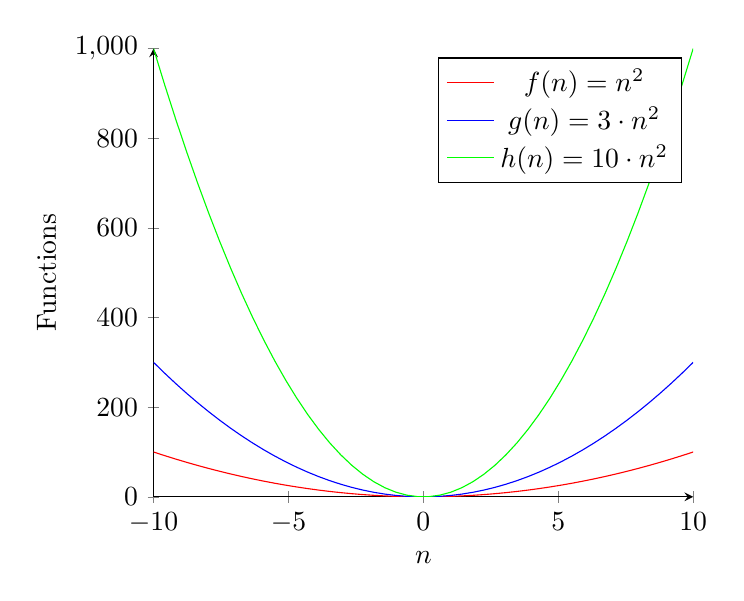
\begin{tikzpicture}
			\begin{axis}[
				axis lines = left,
				xlabel = $n$,
				ylabel = {Functions},
			]
			%Below the red parabola is defined
			\addplot [
				domain=-10:10, 
				samples=50, 
				color=red,
			]
			{x^2};
			\addlegendentry{$f(n) = n^2$}
			%Here the blue parabloa is defined
			\addplot [
				domain=-10:10, 
				samples=50, 
				color=blue,
				]
				{3* x^2};
			\addlegendentry{$g(n) = 3 \cdot n^2$}
			\addplot [
				domain=-10:10, 
				samples=50, 
				color=green,
				]
				{10* x^2};
			\addlegendentry{$h(n) = 10 \cdot n^2$}
			
			\end{axis}
		\end{tikzpicture}
	\end{center}
\end{solution}
\newpage
%Complete the following.
“I have read and agree to the collaboration policy.” -- Isai Lopez Rodas, ilopezro@ucsc.edu
\\
Collaborators: None%write the name of the collaborators. If you worked by yourself, please write 'none'.
\\
\hrule
\item (3 pts) Least counterexample: Give a proof by contradiction using the \emph{least counterexample} method that:
\[
\sum_{i=0}^n i = \frac{n (n+1)}{2}  \qquad \text{for all $n \geq 0$}.
\]
\begin{solution}
	\item
	I will start by providing a base case: i = 0. 
	\begin{equation}\label{eq:14}
		\sum_{i=0}^0 i = \frac{0 (0+1)}{2} = 0
	\end{equation}
	Since we know that the above equation holds true for i = 0, we will assume, for the sake of contradiction, that $\exists\; a \in \mathbb{N}$ such that
	\begin{equation}\label{eq:15}
		\sum_{i=0}^a i \neq \frac{a (a+1)}{2}
	\end{equation}
	In order to show the contradiction, I will now do the summation from $i=0 \rightarrow (a-1)$.
	\begin{equation}\label{eq:16}
		\sum_{i=0}^{a-1} i = \frac{(a-1) ((a-1)+1)}{2} = \frac{(a-1)(a-1+1)}{2} = \frac{(a-1)(a)}{2} = \frac{a^2-a}{2}
	\end{equation}
	I will now add \textnormal{a} to equation \ref{eq:16}
	\begin{equation}\label{eq:17}
		a + \sum_{i=0}^{a-1} i = a + \frac{a^2-a}{2} = \frac{2a}{2} + \frac{a^2-a}{2} = \frac{2a+(a^2-a)}{2}
	\end{equation}
	\begin{equation*}
		= \frac{a^2+2a-a}{2} = \frac{a^2+a}{2} = \frac{a(a+1)}{2} = \sum_{i=0}^{a} i
	\end{equation*}
	Equation \ref{eq:17} shows that adding a to the summation from $i=0 \rightarrow (a-1)$ results in the summation from $i=0 \rightarrow a$. However, this contradicts 
	with our previous statement in equation \ref{eq:15}. Therefore, through a contradiction, we are able to say that the equation $\sum_{i=0}^n i = \frac{n (n+1)}{2}$ holds 
	true for all $n \geq 0$.
\end{solution}
\newpage
\end{enumerate}

\subsection*{Recommended exercises (not to be turned in)}
\begin{enumerate}
\item The solved exercises in Chapters 1, 2, and 5 (Divide and Conquer).
\item Exercises 1 and 2 in Chapter 1 of the text.
\item Exercises 3 and 4 in Chapter 2 of the text.
\end{enumerate} 
\end{document}
